\begin{figure*}[t]
    \centering
    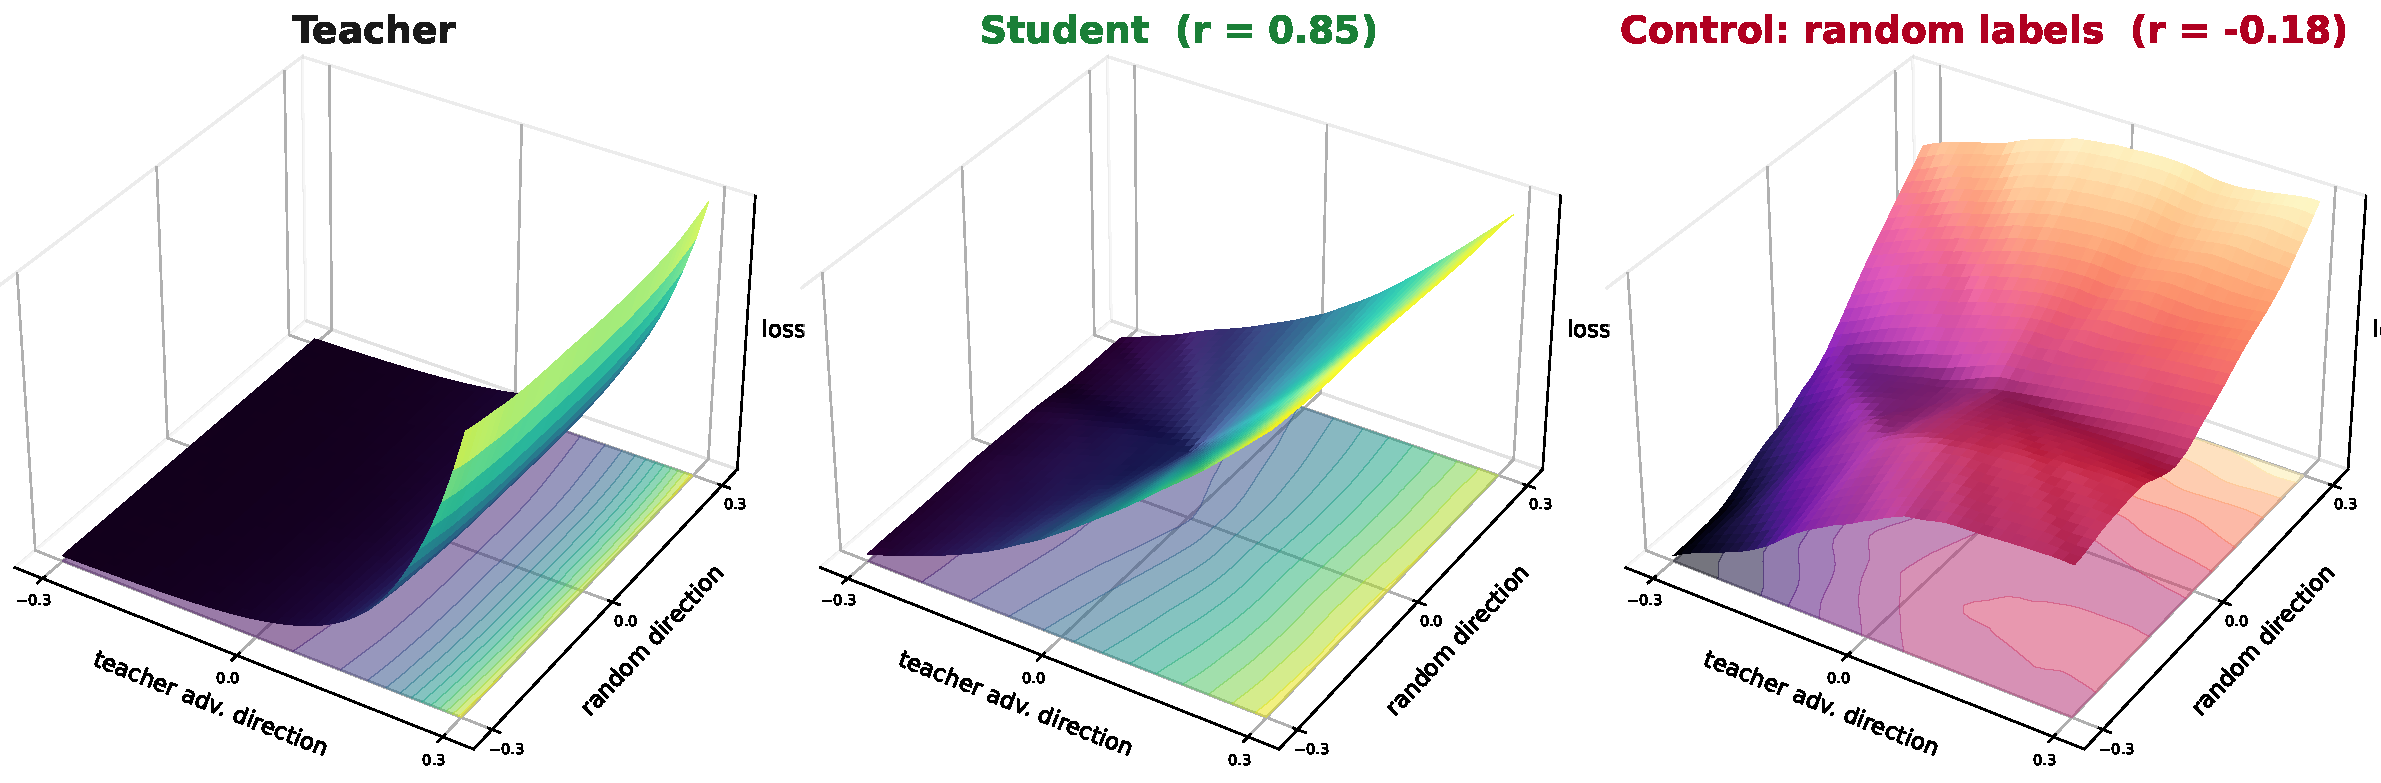
\includegraphics[width=0.95\textwidth]{imgs/teaser_loss_landscape_3d.pdf}
    \caption{Adversarial loss landscapes for a teacher, a student distilled solely on Gaussian noise (no ground-truth labels), and a destroy-the-signal control, evaluated on an MNIST test digit. Each surface plots cross-entropy loss over a $\pm 0.3\,L_{\infty}$ neighborhood spanned by the teacher's adversarial gradient direction and an orthogonal random direction; loss is normalised per panel so shapes are directly comparable. When subliminal learning occurs, the student reproduces the teacher's sharp adversarial ridge $(r = 0.85)$, whereas a control trained identically but on random soft labels does not $(r = -0.18)$ -- showing the adversarial geometry is inherited through the genuine distillation signal rather than the shared architecture or training procedure.}
    \label{fig:teaser_loss}
\end{figure*}